\section{Decision Lists (For CS 6350 students)}
\label{sec:decision-lists}

[20 points] A decision list is an ordered sequence of if-then-else statements. The
sequence of if-then-else conditions are tested in order, and the
answer associated to the first satisfied condition is output.
%
Figure \ref{fig:decision_list} shows an example of a decision list. At
the root of the tree, we check whether $x_1$ is true {\em and} $x_3$
is false. If so, then the label is $0$. Otherwise, we move to the next
node below. Finally, if none of the checks succeed, then the default
label (here $1$ at the bottom of the list) is used.  The specific
decision list here is called a $2$-decision list because no node has
more two conditions to check.


\begin{figure}[h]
\begin{center}
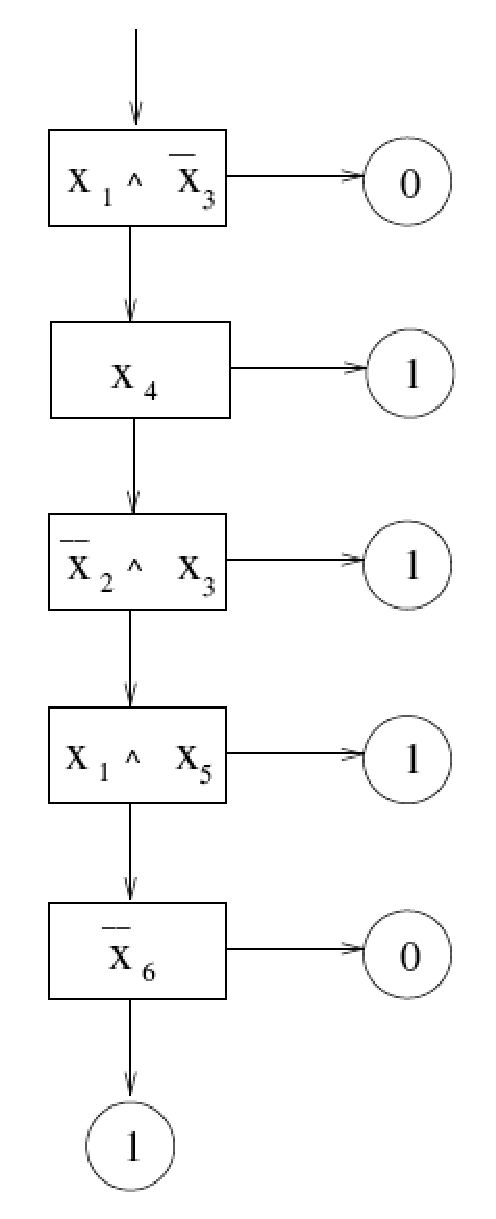
\includegraphics[width=1.35in]{fig-1.pdf}
\caption{A $2$-decision list.}
\label{fig:decision_list}
\end{center}
\end{figure}

Recall from class that a general decision tree can represent
non-linear decision boundaries.  In this question, we are concerned
with a $1$-decision list. Every condition in the $1$-decision list is
either a Boolean variable (such as $x_1$) or a negated Boolean
variable (such as $\neg x_2$). Show that $1$-decision lists are
linearly separable functions.

(Hint: The easiest way to show this is to find a weight vector and a
bias that will make the same predictions as a $1$ decision list. That
is, if the features that are used to construct the decision list are
$\bx = (x_1, x_2, \cdots, x_n)$, then find $\bw$ and $b$ such that the
decision list will return $1$ if, and only if, $\bw^T\bx \geq b$.)



%%% Local Variables:
%%% mode: latex
%%% TeX-master: "hw"
%%% End:
